\chapter{OpenMOLE \& GridScale}

The first part of this chapter expands on the goals, features, architecture and components of the open-source OpenMOLE project. We also explore use cases of the system by looking at a simple workflow. The second part of the chapter describes the structure and design of GridScale, the library OpenMOLE relies on to leverage distributed computing resources from grids and clusters.

\section{OpenMOLE}

OpenMOLE\cite{OpenMOLE} is a workflow execution engine that focuses both on allowing expressive definitions of data processing pipelines and delegation of those tasks to remote execution environments \cite{Leclaire2016}. Compared to other existing workflow management systems like Kepler \cite{Kepler}, Taverna \cite{Taverna}, Galaxy \cite{Galaxy} or Pegasus \cite{Pegasus}, it does not target a specific scientific community and instead aims at offering formalisms that can be used to create generic pipelines.

One of the main objectives of OpenMOLE is embedding workflow models and definitions provided by users in many different forms \cite{Reuillon2013}. Generally, other workflow engines have rigid, text-based rules used to describe individual tasks and their connections, while providing limited support for calling external programs. 

However, OpenMOLE uses a DSL\footnote{Domain Specific Language} built on top of Scala\cite{Scala} to embed a wide variety of tasks defined in any programming language based on the Java Virtual Machine (Java, Scala, Clojure, Groovy, Kotlin). Additionally, prepackaged binaries, C++ executables and Python scripts that depend on shared libraries or pre-loaded packages are seamlessly integrated into workflows. Benefits of relying on Scala's type system include more meaningful task descriptions and early error detection since potential mistakes are caught at compile-time, instead of only after submission to grids or clusters.

Possible execution environments include the user's local machine, SSH servers, grids or self-hosted clusters operated by one of the many supported schedulers: SGE \cite{SGE}, SLURM, PBS \cite{PBS}, HTCondor \cite{HTCondor}, OAR \cite{OAR} or Torque \cite{Torque}. These are all enabled by GridScale \cite{Reuillon2016}, the self-contained library that is shipped by default with OpenMOLE and handles job management on distributed computing environments.

The OpenMOLE platform is now mature and has engaged a loyal user base. It is regularly used for large scale experiments and its robustness in combination with GridScale was proven by experiments where it has been used to run half a billion tasks on EGI\footnote{European Grid Initiative} \cite{Schmitt2015}.

\subsection{Architecture}

The design of the application has been guided by the total decoupling between the creation of the pipelines describing the scientific algorithms and their execution on remote environments \cite{Leclaire2016}. As shown in Figure \ref{OpenMOLEArch}, this led to a layered structure, where the actual experiments are independent from how the tasks they incorporate are run and managed or how the resource requirements are serviced.

\begin{figure}[h]
	\centering
		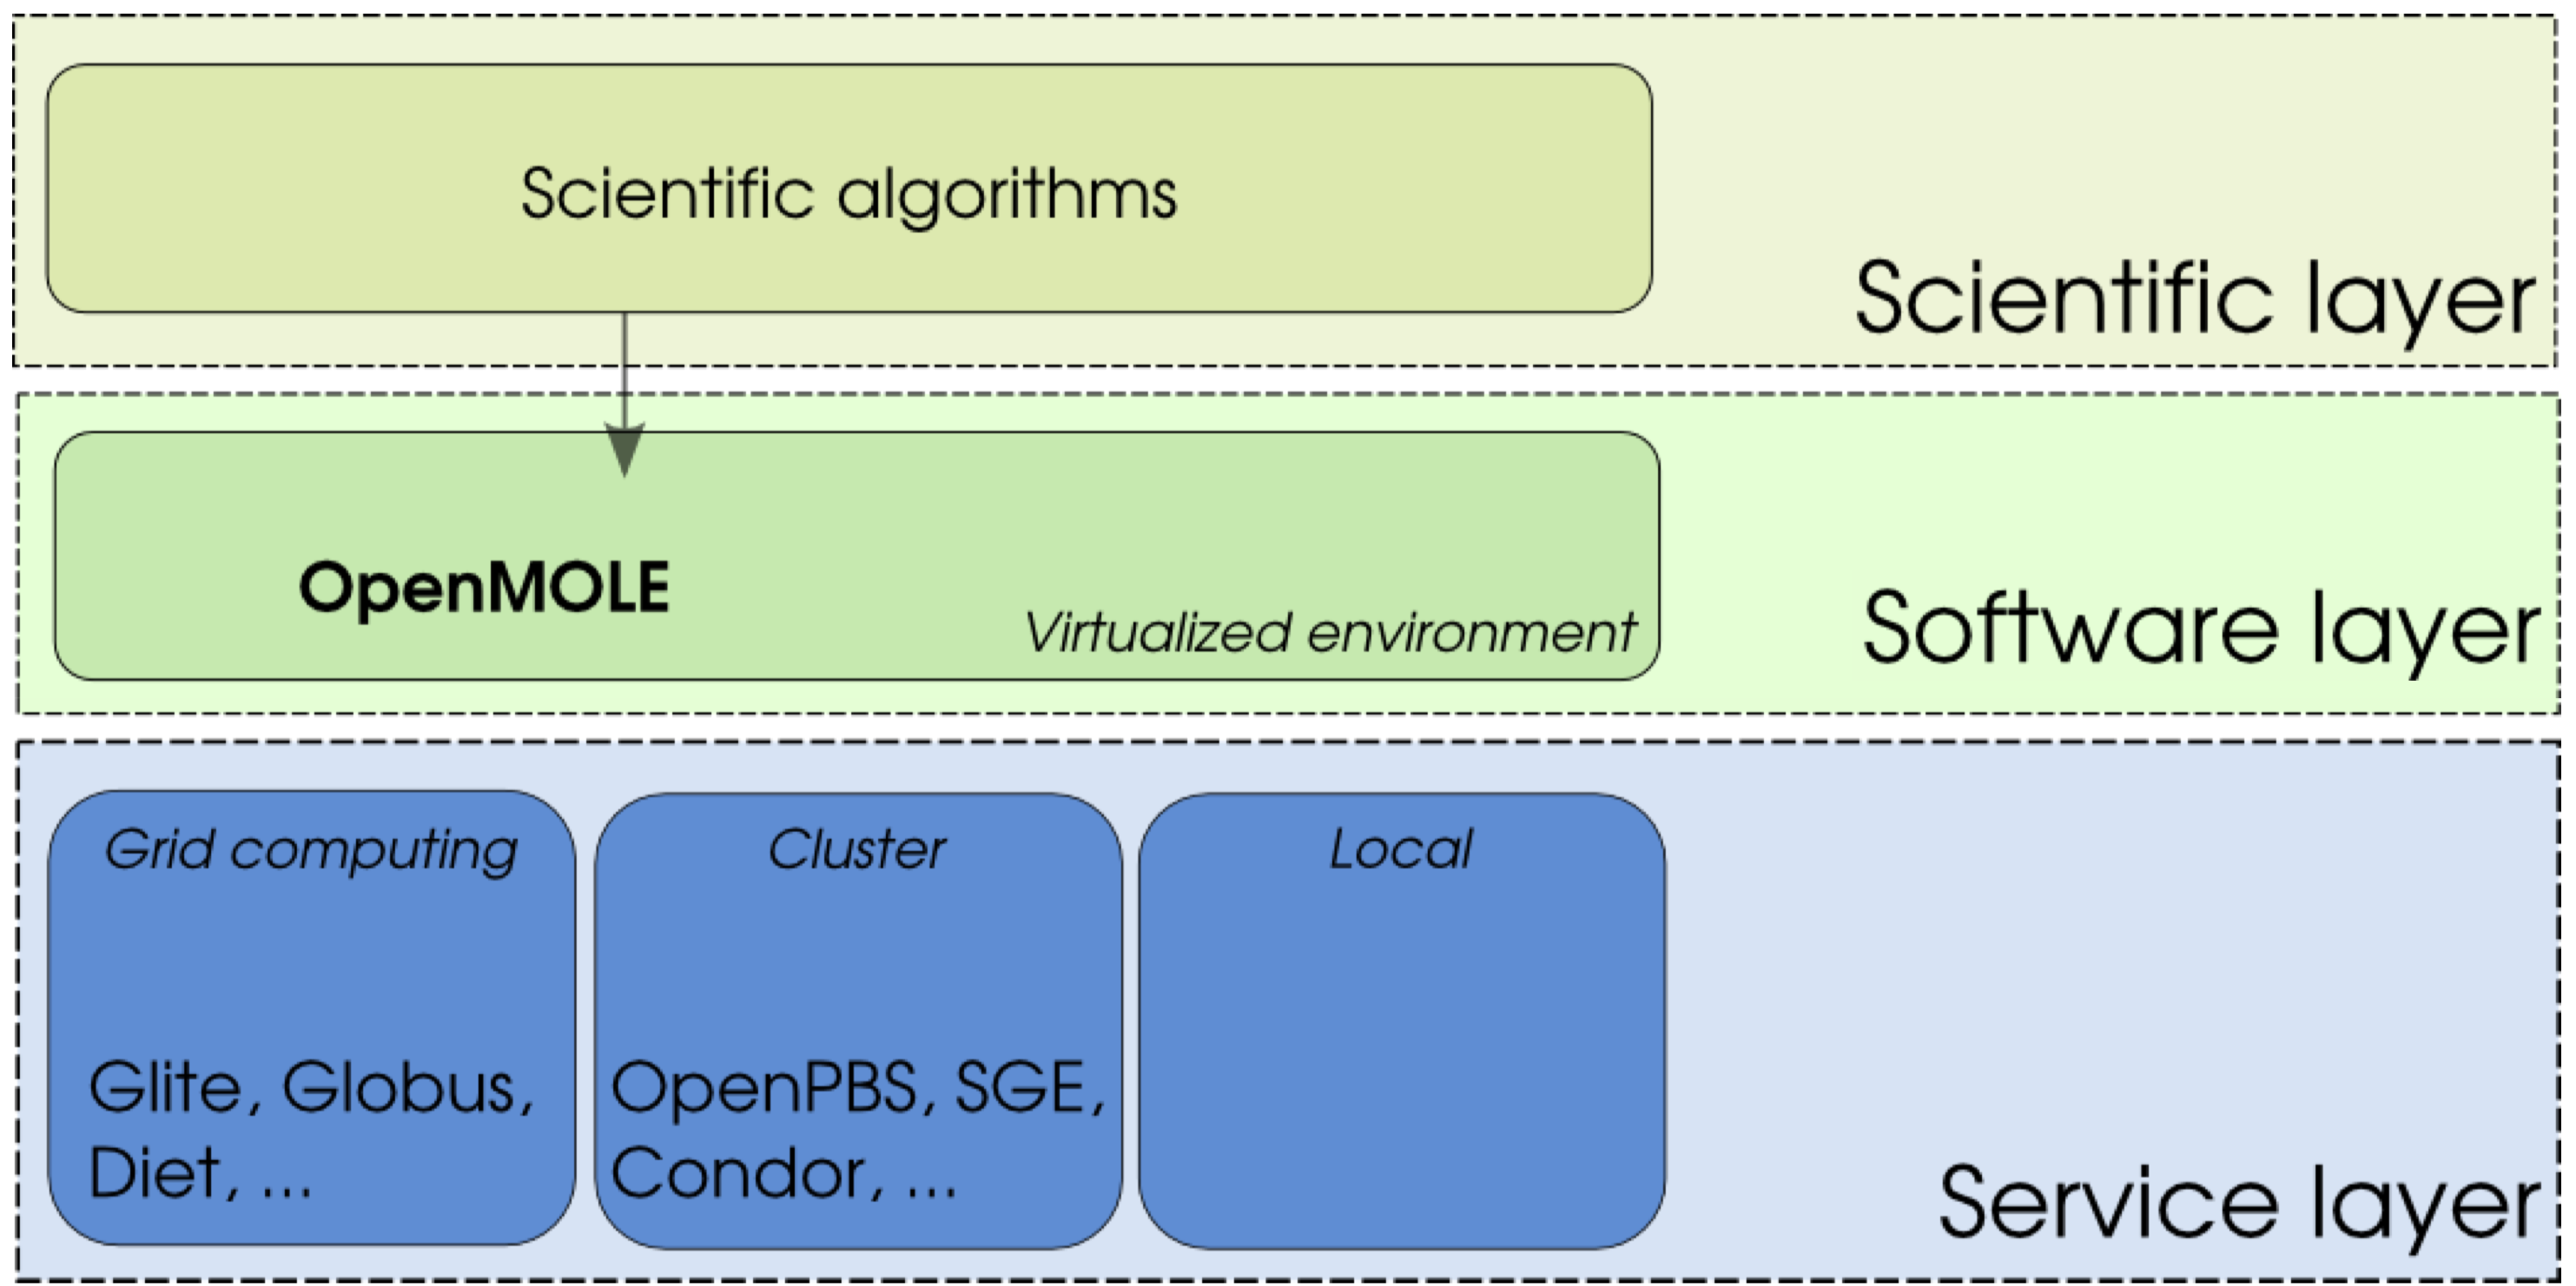
\includegraphics[width=0.9\linewidth]{OpenMOLEArch.png}
	\caption{OpenMOLE layered architecture \cite{Reuillon2010}.}
	\label{OpenMOLEArch}
\end{figure}

In this context, the user is not concerned with how the execution environment is provisioned and can change it easily without altering the workflow description. Additionally, this allows for a fine granularity of task distribution since individual tasks can be sent to environments tailored specifically for their requirements. A clear use case for this are jobs that need to be accelerated using GPUs, with other parts of the workflow running on CPUs as usual.

The structural layers fulfil completely different roles and are modular blocks with clearly defined roles:
\begin{itemize}
	\item The scientific layer relies on the DSL. It is where the user defines the workflow and specifies data sources and execution environments.
	\item The software layer is concerned with the translation of the workflow specification to an internal representation consisting of runnable jobs and their dependencies. It uses the Scala actor model \cite{ScalaActors} to coordinate the whole process of installing the OpenMOLE runtime on each remote execution site, continuously monitoring the status of outstanding jobs, or feeding results of completed tasks to the subsequent ones using them as input. New remote environments are simply added as plugins and they are essentially adapters to the resources exposed by the service layer.
	\item The GridScale library is the service layer, presented in Section \ref{GridScaleSection}.
\end{itemize}

\subsection{Domain Specific Language}

\textit{Tasks} are the basic construct of workflows in OpenMOLE. They essentially consist of a computation that is run against a set of \textit{inputs} to produce a set of \textit{outputs}. Together with \textit{transitions}, which transfer outputs of individual tasks to inputs of subsequent ones, they establish the simplest form of data pipeline.

Listing \ref{SimpleWorkflow} shows a very basic workflow that computes the square of each number from 1 to 100. It begins by declaring variables \verb|i| and \verb|res|, which represent the dataflow and are used to carry results between tasks that are connected via transitions. Since the DSL is build as a set of extensions on top of the Scala programming language, the variables are statically typed, which enables formal verification of the workflow at compile time \cite{Reuillon2013}. This ensures that runtime type mismatches of data transmitted between tasks cannot occur.

\begin{listing}[h]
	\centering
	\begin{minipage}{10.6cm}
		\begin{minted}[frame=single,framesep=2mm,baselinestretch=1.15,fontsize=\small,linenos]{scala}
val i = Val[Int]
val res = Val[Int]

val exploration = ExplorationTask(i in (1 to 100 by 1))

val model =
  ScalaTask("val res = i * i") set (
    inputs += i,
    outputs += (i, res)
  )

val env = LocalEnvironment(8)

exploration -< (model on env hook ToStringHook())
		\end{minted}
	\end{minipage}
	\caption{Simple OpenMOLE workflow.}
	\label{SimpleWorkflow}
\end{listing}

Lines 6-10 define the actual model that we want to compute. In this case, the specification is a \verb|ScalaTask|, where for each input of type \verb|i| the output is a tuple \verb|(i, res)|. Concretely, for input \verb|5|, the output will be \verb|(5, 25)|. Apart from Scala code, a \verb|ScalaTask| can embed code from any programming language running on the JVM (Java, Clojure, Groovy). Other types of tasks include \verb|MoleTask|, used to embed entire predefined workflows, or \verb|CARETask|, used to run any type of prepackaged binary and discussed in section \ref{CARESection}.

One of the central objectives of OpenMOLE is to allow parameter optimisation for the models it executes. The sampling of parameters is achieved through the use of \textit{explorations} in the language. Every parameter sampled from a set is combined with all the other parameters to generate the workflow input. In our case, the exploration at line 4 only samples parameter \verb|i|, so the model will be replicated 100 times and executed with an integer between 1 and 100 as input.


Line 12 instantiates the environment where the workflow will be run. Here we select a \verb|LocalEnvironment| and allow the computation to create and use 8 threads on the local machine. Line 14 ties all the building blocks together. The exploration generates all possible values of \verb|i| and the model is executed on the given environment for each one of them. The \verb|-<| symbol represents a divergent transition between the exploration and the task, each output of the sampling being fed to the model.

In OpenMOLE, \textit{hooks} are used to extract the results of running an experiment. They are executed every time the task that they are assigned to terminates and can perform actions like simply displaying the data or saving it to CSV\footnote{Comma-separated values} files. Here the \verb|ToStringHook| simply prints the output of each task.

Figure \ref{OpenMOLEWorkflow} shows a graphical representation of the combination of primitives described above. This is how a workflow is designed using the graphical user interface instead of the specification language.

\begin{figure}[h]
	\centering
		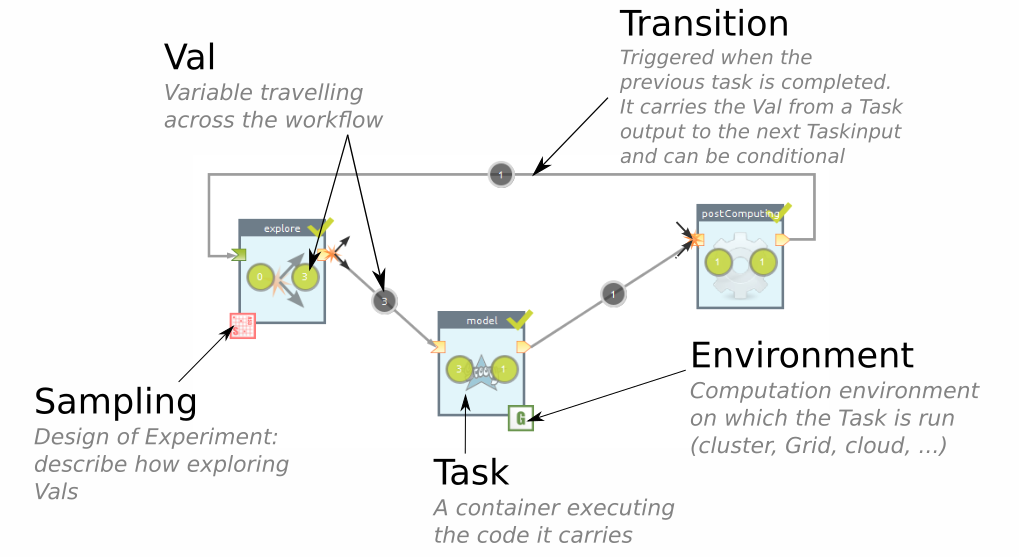
\includegraphics[width=0.8\linewidth]{OpenMOLEWorkflow.png}
	\caption{OpenMOLE workflow \cite{OpenMOLE}.}
	\label{OpenMOLEWorkflow}
\end{figure}

Going beyond the simple example, Listing \ref{Sampling} shows a sampling that explores all combinations of a discrete parameter \verb|i|, a continuous parameter \verb|j|, a file \verb|f| from the given \verb|workDirectory| and a random seed \verb|s| sampled from a uniform distribution. This is achieved using the \textit{x} combinator, which unrolls the domain for each parameter before combining all the possibilities \cite{OpenMOLEDSL}.

\todo[inline]{It's basically a cartesian product of the parameter sets}


\begin{listing}[h]
	\centering
	\begin{minipage}{10.6cm}
		\begin{minted}[frame=single,framesep=2mm,baselinestretch=1.15,fontsize=\small,linenos]{scala}
val i = Val[Int]
val j = Val[Double]
val f = Val[File]
val s = Val[Long]

val exploration = 
  ExplorationTask(
	(i in (0 to 10)) x 
	(j in (0.0 to 100.0 by 10.0)) x
	(f in (workDirectory / "inputs")) x 
	(s in (UniformDistribution[Long]() take 10))
  )
		\end{minted}
	\end{minipage}
	\caption{Advanced exploration \cite{Leclaire2016}.}
	\label{Sampling}
\end{listing}

Listing \ref{Transitions} shows different transitions that can be used to combined task. Note that, for brevity, we did not include any hooks that would collect the results at any stage. 

The execution on line 13 explores the parameter space and feeds each possible value sequentially through each of the 3 tasks. On line 14, \verb|t2| and \verb|t3| are run in parallel on the inputs received from \verb|t1|. Line 15 demonstrates a convergent transition, where the \verb|>-| operator is used to allow an aggregation task to collect and process the results of the run.

\begin{listing}[h]
	\centering
	\begin{minipage}{12.4cm}
		\begin{minted}[frame=single,framesep=2mm,baselinestretch=1.15,fontsize=\small,linenos]{scala}
val i = Val[Int]

val t1 = ScalaTask("i = i * 2") set ( inputs += i, outputs += i )
val t2 = ScalaTask("i = i * 3") set ( inputs += i, outputs += i )
val t3 = ScalaTask("i = i * 4") set ( inputs += i, outputs += i )

val exploration = ExplorationTask( i in (0 to 100) )
val aggregate = ScalaTask("val i = input.i.sum") set (
  inputs  += i.toArray,
  outputs += i
)

exploration -< t1 -- t2 -- t3
exploration -< t1 -- (t2, t3)
exploration -< t1 -- t2 -- t3 >- aggregate
		\end{minted}
	\end{minipage}
	\caption{Transition types \cite{OpenMOLEDSL}.}
	\label{Transitions}
\end{listing}

Our initial example showed the simple case of running a workflow on the user's machine using a \verb|LocalEnvironment|. However, this is only usually done for testing locally before scaling the experiment and other types of environments are used for real experiments. Listing \ref{Environments} shows examples of instantiating SSH servers and cluster environments.

The user can be authenticated either with a login and password combination, or via a private key. Here we define the authentication by specifying the path to the private key, the associated login and the remote machine's full address. The \verb|encrypted| parameter references a function that will prompt the user for the key's password in case it is protected.

Environments are created by providing the shell login on the remote machine and its address. For the SSH server, we also specify the number of cores that can be used by the workflow. Cluster environments require that the target machine can act as the master of the cluster, being able to take commands for submitting and querying job status.

\begin{listing}[h]
	\centering
	\begin{minipage}{11.5cm}
		\begin{minted}[frame=single,framesep=2mm,baselinestretch=1.15,fontsize=\small,linenos]{scala}
SSHAuthentication += 
  PrivateKey(
    "path/to/private/key",
    "login",
    encrypted, 
    "machine-address")

val sshEnv = SSHEnvironment("login", "machine-address", 8)
val condorEnv = CondorEnvironment("login", "master-address")
val sgeEnv = SGEEnvironment("login", "master-address")
		\end{minted}
	\end{minipage}
	\caption{Usage of various environments.}
	\label{Environments}
\end{listing}

The aim is to provide a similar \verb|AWSEnvironment| primitive, which only receives the user's AWS credentials as parameters. This should automatically create a cluster backed up by EC2 instances and configure it with a scheduler that distributes job submissions generated by the workflow.


\todo[inline]{You need to highlight that even more as it's the take home message for this section: "here is litterally what we want to do!"}

\subsection{Job Distribution}

Compared to other workflow platforms, OpenMOLE follows a zero-deployment approach, meaning that it does not rely on any software being installed on the target machines that the task-generated jobs will run on \cite{Reuillon2013}. In order to support this, a setup phase is required before the task execution step itself. This involves uploading several components to the remove environment \cite{Reuillon2010}:

\begin{itemize}
	\item The OpenMOLE runtime, which includes the OpenMOLE framework and the Java Virtual Machine used to run it.
	\item Task descriptions along with their serialized execution contexts, which describe variables used by the task to transport data.
	\item Resource files used by the tasks.
\end{itemize}

After all the dependencies are in place, a job is packaged to reference the runtime, task and context it corresponds to. Once it is assigned to an execution node by the environment's native submission system, it downloads the runtime and runs the task in the given context. Note that the potentially expensive step of copying the runtime on each node is rarely necessary in practice, since clusters and grids usually operate on filesystems shared across all nodes. OpenMOLE also maintains a cache of the file replicas already uploaded to remote storages, so that a file never gets uploaded twice to the same storage as long as it's not been modified on the host system.

Once finished, jobs upload their results to the storage system. Meanwhile, the OpenMOLE framework continuously tracks the state of the job by querying the submission system and downloads the outputs on the local machine of the user upon completion. The whole process is presented as a sequence diagram in Figure \ref{OpenMOLERuntime}.

\begin{figure}[H]
	\centering
		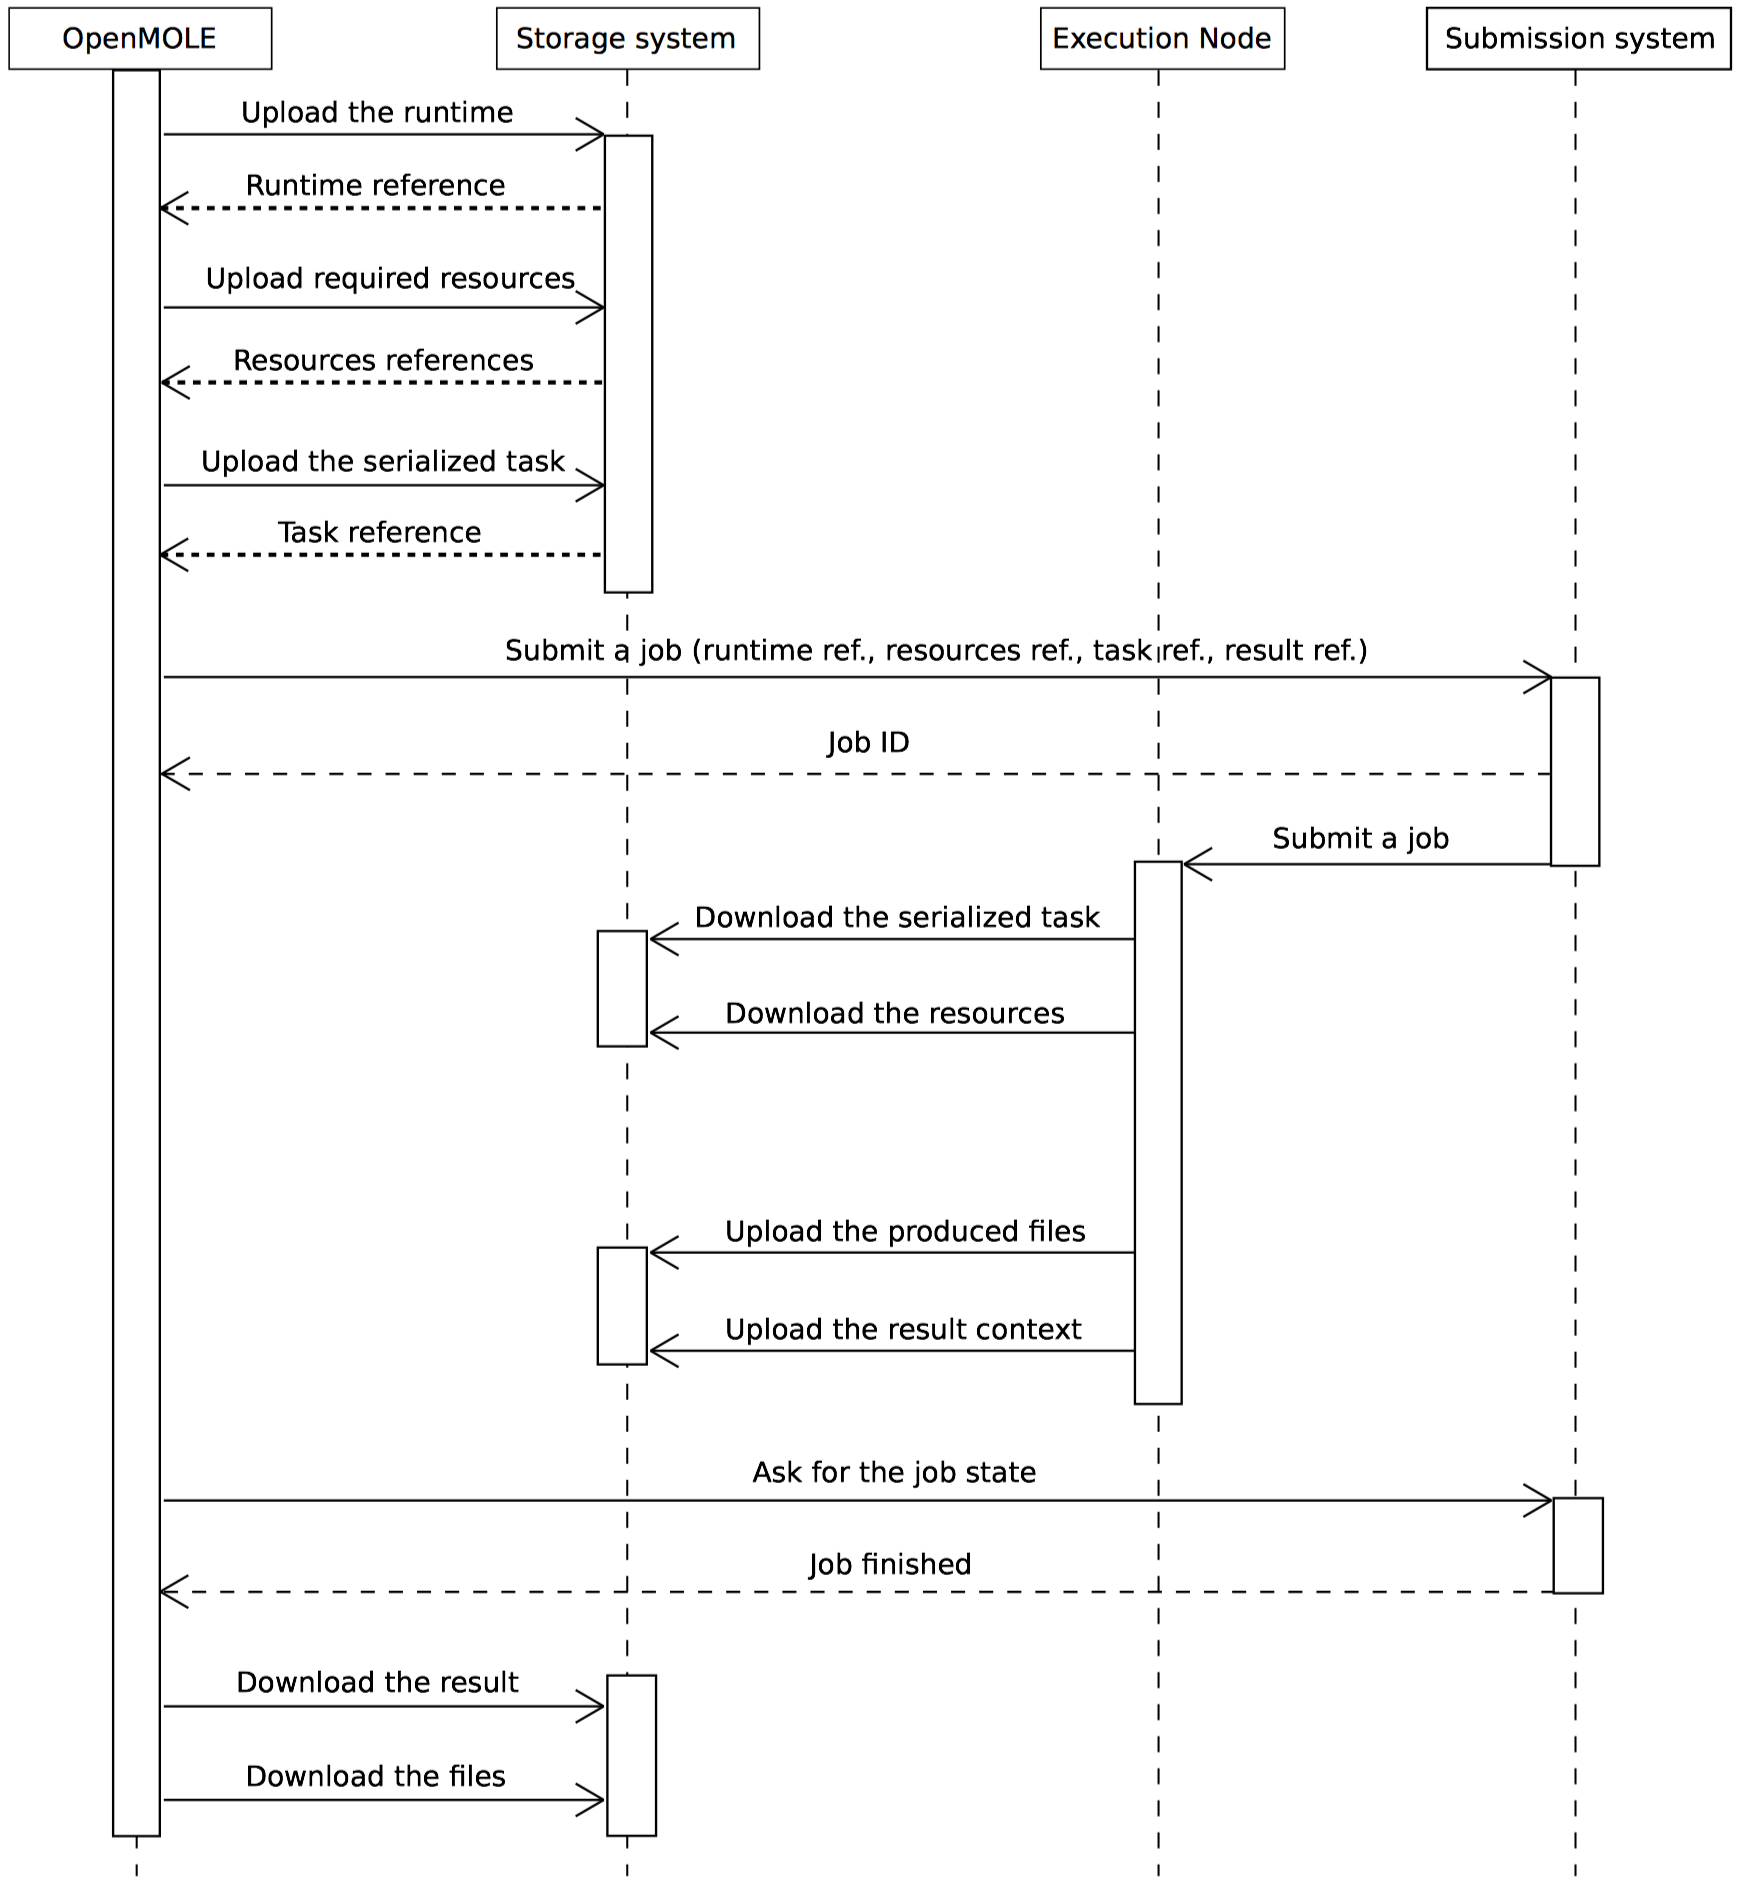
\includegraphics[width=1\linewidth]{OpenMOLERuntime.png}
	\caption{Delegation of a task to remote execution environment in OpenMOLE. \cite{Reuillon2010}.}
	\label{OpenMOLERuntime}
\end{figure}

\subsection{CARE} \label{CARESection}

\begin{figure}[h]
	\centering
		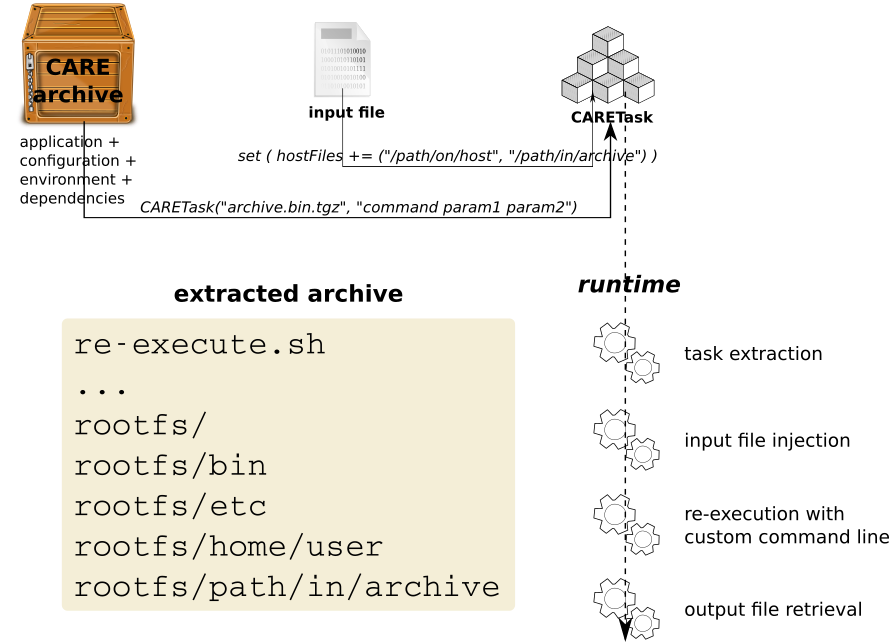
\includegraphics[width=0.9\linewidth]{OpenMOLECARE.png}
	\caption{Delegation of a task to remote execution environment in OpenMOLE. \cite{Leclaire2016}.}
	\label{OpenMOLECARE}
\end{figure}

\subsection{Code Structure}

\section{GridScale} \label{GridScaleSection}